\section{问题重述}
\subsection{问题背景}

待调度的对象是由操作节点和张量节点交替连接而成的有向无环计算图。操作表示一次计算或数据搬运，张量表示其输入、中间结果或输出；两者之间的有向边规定了操作何时才能开始。对于分块神经网络计算，一个计算块可能先由外部存储器搬入核内，再由矩阵或向量单元处理，最后将结果写回外部存储器。多个块的依赖、共享输入和中间张量驻留同时存在，因此仅按操作数平均分配到各核，不能保证总完成时间缩短。

神经网络处理器研究已有对硬件平台、体系结构及降低计算成本路径的系统综述\cite{sze2017}。Eyeriss 对局部复用和片外访存能耗的实证分析说明，数据流设计会显著改变搬运代价\cite{eyeriss2017}；TPU 的整模型评估则提醒我们，专用矩阵单元的峰值能力不能单独代表应用完成时间\cite{jouppi2017}。经典的红蓝卵石模型从理论上刻画有限快存下计算与I/O的牵制\cite{hongkung1981}。这些研究提供背景，本题的数值结果仍以题给评估语义为准。

题目给定的平台由若干同构 NPU 核心及共享 DDR 组成。每个核心具备矩阵、向量和两类数据搬运流水线，同时有私有 L1 与 UB 缓存；各核的 DDR 读写争用同一物理带宽。跨核并行可分担计算，但张量一旦跨越不能直接复用的边界，就可能增加读写与同步等待。反过来，过度合并虽然减少边界，却会拉长单个核心的计算段，并使中间张量占据缓存更久。切图、分核和核内顺序由此相互牵制。

这种牵制还取决于硬件组织。无核间同步机制时，每个子图作为单独 Task 下发，同核相邻 Task 也不能保留前一 Task 的私有缓存；有同步机制时，同核多个子图可合成一个 Task，保留部分中间数据，但跨核张量仍需经 DDR 中转。后者可能节省边界读写，也可能让长时间驻留的张量挤占缓存。进一步引入共享只读 L2 后，多核重复读取的部分输入有机会改由 Cache 服务，而命中率又受容量、FIFO 淘汰顺序和读带宽约束。这三种条件需要按各自真实规则评价。

本题提供完整计算图、容量与带宽配置、合法方案格式，以及包含核内排布和多核事件模拟的评估程序。评估程序会根据子图边界补充搬运、在必要时插入缓存换入换出，并在共享带宽争用下重算全局操作完成时刻。因此，单独的拓扑层数、各核工作量总和或核内参考时间都不能直接充当最终 Makespan。研究需要同时保证方案覆盖与依赖合法、私有存储不越界、全局执行能结束，并在相同的官方配置下比较总时长和新增搬运量。

\subsection{问题重述}

对每个给定计算图，需要把全部非 COPY 操作映射到子图编号，把每个子图恰好安排到一个核心，并给出同核子图的执行顺序。子图依赖图不得有环，顺序不得违反依赖；方案交由题目规定的评估流程确定核内操作序、缓存换入换出和共享资源上的实际时间线。核心数量变化时，方法仍应在合理时间内产生可执行方案。评价以全局 Makespan 为主，同时控制相对原始图增加的 DDR 搬运字节数。

问题一针对场景 A：一个子图就是一个 Task，跨子图张量都须经 DDR；跨核前驱 Task 与同核 Task 切换分别受题定等待时间约束。应建立切图和调度模型，分别为二至五核生成方案。正文需展示以整图单核时长为基准的一至五核平均加速比，逐例结果表列出全部给定算例的官方 Makespan 与额外搬运量，并保留可复现程序和方案文件。

问题二针对场景 B：同核全部子图合为一个 Task，可在 L1 或 UB 中复用数据，跨核依赖则以 DDR 拷贝和固定同步延迟实现。需在满足每核私有缓存容量的前提下，调整切图、分核与顺序，在二至五核稳定生成方案，争取进一步降低全局时长和额外搬运。其平均加速比仍以与问题一相同的整图单核结果为分母；逐例指标与方案同样须保留在支撑材料中，并提供可复现的 Python 程序。

问题三在场景 B 上增加所有核心共享的只读 L2。只有 COPY\_IN 查询 Cache；命中不改变 FIFO 顺序，L2 读带宽与 DDR 带宽独立。需研究容量与读带宽变化如何影响切图、调度及完成时间，设计相应方案，并在题定容量和带宽下完成全部正式用例。正文比较同核数无 L2 与有 L2 的结果，Cache 加速比须在同一方案上用无 L2 时长除以有 L2 时长；逐例结果表列出两种配置的 Makespan、额外搬运量和命中率。

本文的研究安排如图~\ref{fig:roadmap} 所示。

\begin{figure}[htbp]
  \centering
  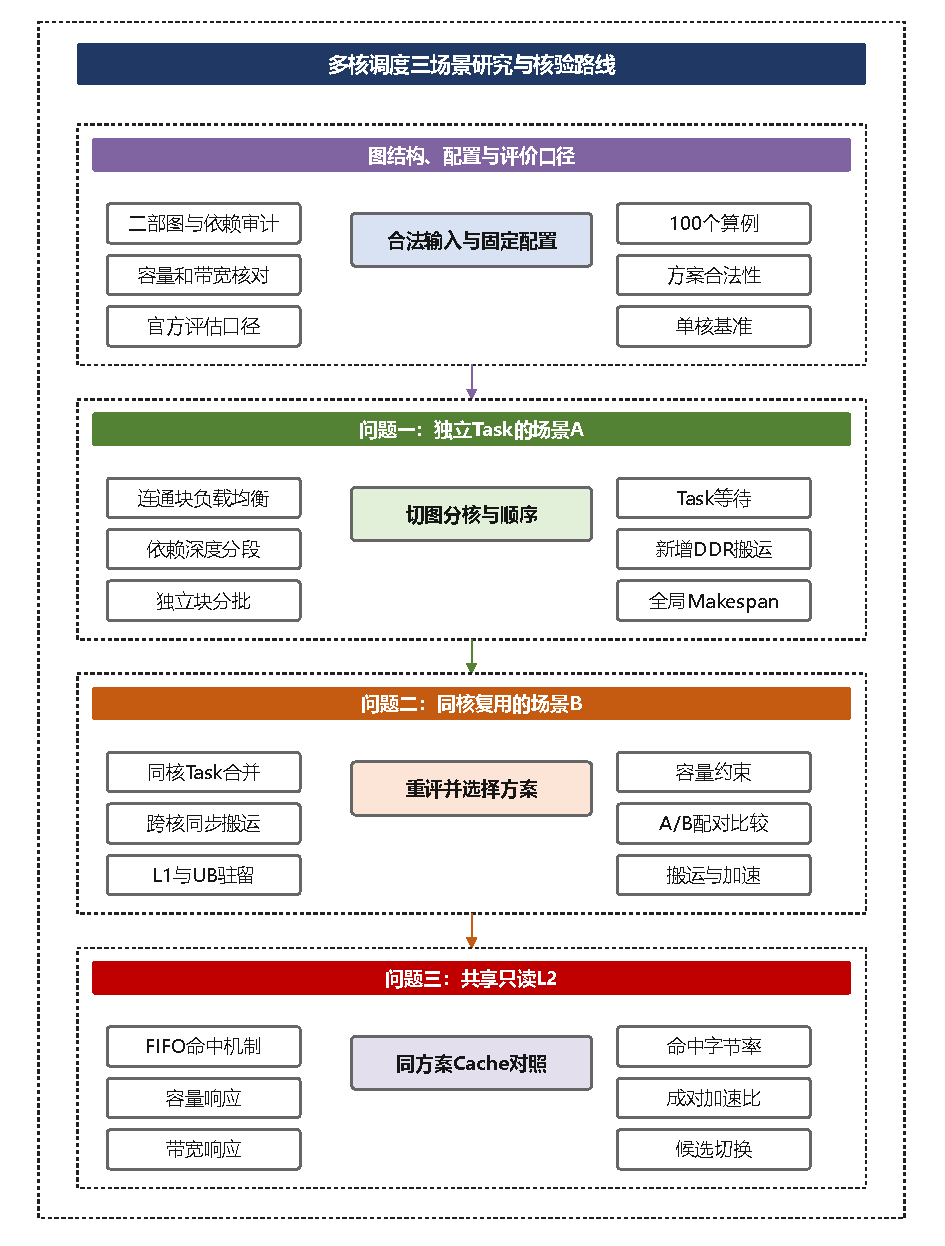
\includegraphics[width=160mm]{../求解/总体路线图_论文宽.pdf}
  \caption{多核调度研究路线}
  \label{fig:roadmap}
\end{figure}

\FloatBarrier

路线图先核查图结构、配置及评估口径，再依照场景 A、场景 B 和共享 L2 的条件组织候选方案与合法性验证，最后用同一批官方算例比较速度、搬运和缓存响应。这一路线是本文的求解安排，并不改变题目对三个问题的交付要求。


